% Created 2021-09-27 Mon 11:52
% Intended LaTeX compiler: xelatex
\documentclass[letterpaper]{article}
\usepackage{graphicx}
\usepackage{grffile}
\usepackage{longtable}
\usepackage{wrapfig}
\usepackage{rotating}
\usepackage[normalem]{ulem}
\usepackage{amsmath}
\usepackage{textcomp}
\usepackage{amssymb}
\usepackage{capt-of}
\usepackage{hyperref}
\setlength{\parindent}{0pt}
\usepackage[margin=1in]{geometry}
\usepackage{fontspec}
\usepackage{svg}
\usepackage{cancel}
\usepackage{indentfirst}
\setmainfont[ItalicFont = LiberationSans-Italic, BoldFont = LiberationSans-Bold, BoldItalicFont = LiberationSans-BoldItalic]{LiberationSans}
\newfontfamily\NHLight[ItalicFont = LiberationSansNarrow-Italic, BoldFont       = LiberationSansNarrow-Bold, BoldItalicFont = LiberationSansNarrow-BoldItalic]{LiberationSansNarrow}
\newcommand\textrmlf[1]{{\NHLight#1}}
\newcommand\textitlf[1]{{\NHLight\itshape#1}}
\let\textbflf\textrm
\newcommand\textulf[1]{{\NHLight\bfseries#1}}
\newcommand\textuitlf[1]{{\NHLight\bfseries\itshape#1}}
\usepackage{fancyhdr}
\pagestyle{fancy}
\usepackage{titlesec}
\usepackage{titling}
\makeatletter
\lhead{\textbf{\@title}}
\makeatother
\rhead{\textrmlf{Compiled} \today}
\lfoot{\theauthor\ \textbullet \ \textbf{2021-2022}}
\cfoot{}
\rfoot{\textrmlf{Page} \thepage}
\renewcommand{\tableofcontents}{}
\titleformat{\section} {\Large} {\textrmlf{\thesection} {|}} {0.3em} {\textbf}
\titleformat{\subsection} {\large} {\textrmlf{\thesubsection} {|}} {0.2em} {\textbf}
\titleformat{\subsubsection} {\large} {\textrmlf{\thesubsubsection} {|}} {0.1em} {\textbf}
\setlength{\parskip}{0.45em}
\renewcommand\maketitle{}
\author{Houjun Liu}
\date{\today}
\title{Trajectories!}
\hypersetup{
 pdfauthor={Houjun Liu},
 pdftitle={Trajectories!},
 pdfkeywords={},
 pdfsubject={},
 pdfcreator={Emacs 28.0.50 (Org mode 9.4.4)}, 
 pdflang={English}}
\begin{document}

\tableofcontents


\section{Derived Equations of Kinematics}
\label{sec:orgf07c745}
Just for review: 

\begin{equation}
    \begin{cases}
        x(t) = x_0 + v_0 t + \frac{1}{2} a_0 t^2 \\
        v(t) = v_0 + a_0 t \\
        v^2(x) = {v_0}^2 + 2a(x-x_0) \\
        v_{av} = v_{av}\Delta t
    \end{cases}
\end{equation}

Where,
\begin{equation}
    \begin{cases}
        v_{av} = \frac{1}{2}(v_1+v_2) \\
        \Delta x = x_2-x_1 \\
        \Delta t = t_2-t_1
    \end{cases}
\end{equation}

\section{Projectile Problem}
\label{sec:orgbfc102d}

\subsection{Proving that \(R = \frac{2sin(2\theta){v_0}^2}{g}\)}
\label{sec:orgb1f12e2}
We begin by establishing the figure by which this model is based on:

\begin{center}
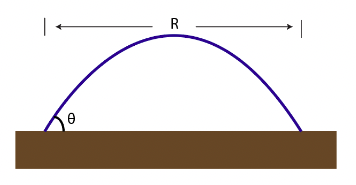
\includegraphics[width=.9\linewidth]{2021-09-14_18-52-12_screenshot.png}
\end{center}


We set the velocity at which the launcher launches object is launched from as \(v_0\). Furthermore, we set the initial time at which the object is launched as \(t_0\), the initial position of the trajectory as \((x_0, y_0)\), the final position of the trajectory as \((x_f,y_f)\). We will, as with tradition, set the acceleration due to gravity as \(g\).

To begin, we will create some basic assumptions and statements that we could make given the setup of the problem:

\begin{equation}
    \begin{cases}
        x_0 = 0 \\
        y_0 = 0 \\
        x_f = R \\
        y_f = 0 \\
    \end{cases}
\end{equation}

These assumptions indicate that the object starts by being launched at a position we denote as \((0,0)\) in the system, and travels right (to the positive direction, under current system) such that --- after a presumably parabolic trajectory --- it reaches position \((R,0)\): \(R\) units out and on the ground \(y=0\) again.

We begin approaching this problem by separating out the third equation of kinematics (relating to position) into a set of parametric equations involving the \(x\) and \(y\) positions as separate parameters. That is,

\begin{equation}
    \begin{cases}
        x(t) = \frac{-1}{2}g_xt^2 + v_0\cos\theta t + x_0 \\
        y(t) = \frac{-1}{2}g_yt^2 + v_0\sin\theta t + y_0 
    \end{cases}
\end{equation}

Therefore, replacing the assumptions regarding the start positions, we could therefore make the following statements regarding the end position of the projectile:

\begin{equation}
    \begin{cases}
        x_f = R = \frac{-1}{2}g_x{t_f}^2 + v_0\cos\theta t_f \\
        y_f = 0 = \frac{-1}{2}g_y{t_f}^2 + v_0\sin\theta t_f
    \end{cases}
\end{equation}

However, we could simplify this statement even further by the realization that, under the current axis system, there is \emph{no} x-component acceleration due to gravity (that is, \(g_x = 0\).) With this claim, we conclude that:

\begin{equation}
    \begin{cases}
        x_f = R = v_0\cos\theta t_f \\
        y_f = 0 = \frac{-1}{2}g{t_f}^2 + v_0\sin\theta t_f
    \end{cases}
\end{equation}

The goal for this deduction is to figure a function \(R\) --- distance traveled of projectile --- given angle \(\theta\). Hence, a good method by which this system could be combined into one statement is by performing variable substitution upon \(t_f\), hence eliminating time as a variable in the system and combining the two statements.

We first transpose the first statement such that it is w.r.t. \(t_f\):

\begin{align}
    &R = v_0 \cos\theta t_f \\
\Rightarrow &\frac{R}{v_0 \cos\theta} = t_f
\end{align}

Substituting this resulting expression into the statement for \(y_f\), and simplifying, we deduct that:

\begin{align}
    0 =& \frac{-1}{2}g(\frac{R}{v_0 \cos\theta})^2 + v_0 \sin\theta (\frac{R}{v_0 \cos\theta}) \\
    0 =& \frac{-1}{2}g\frac{R^2}{{v_0}^2 \cos^2\theta} + \tan\theta R \\
    0 =& R (\frac{-1}{2}g\frac{R}{{v_0}^2 \cos^2\theta} + \tan\theta) \\
\end{align}

Given this expression, we could deduct two statements of the roots of this function w.r.t. \(R\):

\begin{equation}
    \begin{cases}
        0 = R \\
        0 = \frac{-1}{2}g\frac{R}{{v_0}^2 \cos^2\theta} + \tan\theta
    \end{cases}
\end{equation}

A \(R\) represents the total distance traveled \emph{after} the projectile motion, we disregard the first case and proceed to isolate \(R\) in the latter case.

\begin{align}
    0 =& \frac{-1}{2}g\frac{R}{{v_0}^2 \cos^2\theta} + \tan\theta \\
    \Rightarrow 2\tan\theta =& g\frac{R}{{v_0}^2 \cos^2\theta} \\
    \Rightarrow \frac{2\tan\theta}{g} =& \frac{R}{{v_0}^2 \cos^2\theta} \\
    \Rightarrow R =& \frac{2\tan\theta {v_0}^2 \cos^2\theta}{g} \\
    \Rightarrow R =& \frac{2\frac{\sin\theta}{\cos\theta} \cos^2\theta {v_0}^2}{g} \\
    \Rightarrow R =& \frac{2\sin\theta\cos\theta {v_0}^2}{g} \\
\end{align}
At this point, we apply the following Double Angle Formulae:

\begin{equation}
    sin(2\theta)=2\sin\theta\cos\theta
\end{equation}

Which would simplify the resulting expression to:

\begin{equation}
    R = \frac{2sin(2\theta){v_0}^2}{g}
\end{equation}

\subsection{Maximizing \(R(\theta)\)}
\label{sec:orgffe34f0}
Given\ldots{}

\begin{equation}
    R(\theta) = \frac{2sin(2\theta){v_0}^2}{g}
\end{equation}

there are two ways by which \(\theta=45^{\circ}=\frac{\pi}{4}rad\) could be determined to be a local maximum of \(R(\theta)\).

\subsubsection{\ldots{}via sinusoidal periods}
\label{sec:org2eb0cf0}
The function \(R(\theta)\) is predicated upon one independent variable: that of \(\theta\). It appears once in the expression for \(R(\theta)\), in the term \(\sin(2\theta)\).

To maximize \(R(\theta)\), therefore, \(\sin(2\theta)\) must be maximized. The sine function is sinusoidal (definitely so), and hence its range is \([-1, 1]\). Its maximum value is therefore \(\sin(2\theta) = 1\).

Hence, we could figure the value of \(2\theta\) provided that we are limited to one period \(0\leq 2\theta \leq 2\pi\).

\begin{align}
    1 =& \sin(2\theta) \\
    \Rightarrow 2\theta =& \arcsin(1) \\
    \Rightarrow 2\theta =& \frac{\pi}{2} \\
    \Rightarrow \theta =& \frac{\pi}{4} 
\end{align}

Hence, \(\theta=\frac{\pi}{4}rad=45^{\circ}\) for \(R(\theta)\) to be maximized.

\subsubsection{\ldots{}via critical points}
\label{sec:org3bc4d0c}
Local maximums of \(R(\theta)\) appears at critical points of \(R(\theta)\) where \(R'(\theta)\) changes signs from positive to negative. To figure this, we first find the critical points of \(R(\theta)\) via the first derivative test.

First, we figure the first derivative of this function:

\begin{align}
    R(\theta) =& \frac{2\sin(2\theta){v_0}^2}{g} \\
    \Rightarrow \frac{d}{d\theta} R(\theta) =& \frac{d}{d\theta} \frac{2sin(2\theta){v_0}^2}{g} \\
    \Rightarrow \frac{d}{d\theta} R(\theta) =& \frac{2{v_0}^2}{g} \frac{d}{d\theta} \sin(2\theta) \\
    \Rightarrow \frac{d}{d\theta} R(\theta) =& \frac{2{v_0}^2}{g} 2\cos(2\theta) \\
\end{align}

To apply the first derivative test, we set this expression equal to \(0\) and solve for \(\theta\).

\begin{align}
    R(\theta) =& \frac{2{v_0}^2}{g} 2\cos(2\theta) \\
\Rightarrow 0 =& \frac{2{v_0}^2}{g} 2\cos(2\theta) \\
\Rightarrow 0 =& \underbrace{\frac{2{v_0}^2}{g}2}_{not\ involving\ \theta} \cos(2\theta) \\
\Rightarrow 0 =& \cos(2\theta) \\
\end{align}

If we again limit ourselves to one period \(0\leq 2\theta \leq 2\pi\), \(cos(2\theta)\) takes on the value of \(0\) at \(\theta = \frac{\pi}{4}\) and \(\theta = \frac{-\pi}{4}\).

In the latter case, the second derivative function travels from negative to positive --- making it a local \emph{minimum}, which is not the point we are seeking. The former case does satisfy the transition between positive to negative: making it, per the first derivative test, a local maximum.

Hence, \(\theta=\frac{\pi}{4}rad=45^{\circ}\) for \(R(\theta)\) to be maximized.

\section{Collision Problem}
\label{sec:org1cfd19e}
Prove that, when an object is dropped and another fired, they will collide as long as the projectile is aimed at the target and reaches the vertical path of the target regardless of the launch velocity.

\subsection{Modeling Collision}
\label{sec:orgbb08e20}
We set the projectile to be \(m_1\), and the vertically dropping object to be \(m_2\). We also define the horizontal distance of the x-components between \(m_1\)'s start's position and \(m_2\) as \(x_0\). Furthermore, we set the initial height of \(m_2\) as \(h_0\). We set height of the collision location as \(h\).

For the two objects to collide at a time \(t_1\), they have to share x and y coordinate values. Meaning, both components of their equation of kinematics regarding position have to match. To figure such a \(t_1\), we first set up two sets of equations for kinematics that would model the situation.


\subsubsection{To model \(m_1\)\ldots{}.}
\label{sec:org6fd01fe}
We begin with the equations of kinematics revised for this situation:

\begin{equation}
    \begin{cases}
        x(t) = v_0\cos\theta t \\
        y(t) = \frac{-1}{2}g t^2 + v_0\sin\theta t
    \end{cases}
\end{equation}

As with the last problem, we notice that \(g_x=0\) because there is no x-component acceleration due to gravity under our system. Furthermore, there are no constants in the initial state of this model due to our definition of the projectile being at \((0,0)\) at the start of the experiment.

Due to the fact that we know \(m_1\) is aimed towards the object, we know that the projectile is aimed such that \(\tan(\theta) = \frac{h_0}{x_0}\) ("up towards object, that's right facing \(x_0\) away"). Hence, \(\theta = \tan^{-1}(\frac{h_0}{x_0})\). 

\begin{equation}
    \begin{cases}
        x(t_1) = v_0\cos(\tan^{-1}(\frac{h_0}{x_0}))t_1 \\
        y(t_1) = \frac{-1}{2}g {t_1}^2 + v_0\sin(\tan^{-1}(\frac{h_0}{x_0})) t_1
    \end{cases}
\end{equation}


\subsubsection{To model \(m_2\)\ldots{}.}
\label{sec:orgc3516e1}
As similar to before, we begin with the equations of kinematics for \(m_2\)'s situation:

\begin{equation}
    \begin{cases}
        x(t) = x_0 \\
        y(t) = \frac{-1}{2}g{t}^2 + y_0
    \end{cases}
\end{equation}

We again notice that \(g_x=0\) due to the same line of reasoning. In fact, as the x-component of position of \(m_2\) never changes, it stays constant at \(x_0\).

We also notice that, as the object is simply in free fall, there is no \(v_0\) to be had initially. Hence, that term is set to \(0\) as well. Furthermore, as part of the setup of the problem, the falling object starts its fall at a height \(h\).

\begin{equation}
    \begin{cases}
        x(t_1) = x_0 \\
        y(t_1) = \frac{-1}{2}g{t_1}^2 + h_0
    \end{cases}
\end{equation}

\subsubsection{Modeling the process of fall}
\label{sec:org9644857}
Given the two systems determined for \(m_1\) and \(m_2\) respectively:

\begin{equation}
    \begin{cases}
        x(t_1) = v_0\cos(\tan^{-1}(\frac{h_0}{x_0}))t_1 \\
        y(t_1) = \frac{-1}{2}g {t_1}^2 + v_0\sin(\tan^{-1}(\frac{h_0}{x_0})) t_1
    \end{cases}
\end{equation}

\begin{equation}
    \begin{cases}
        x(t_1) = x_0 \\
        y(t_1) = \frac{-1}{2}g{t_1}^2 + h_0
    \end{cases}
\end{equation}

For the objects to collide, these two systems must equal to each other. Setting them so\ldots{}

\begin{equation}
    \begin{cases}
        x_0 = v_0\cos(\tan^{-1}(\frac{h_0}{x_0}))t_1\\
        \frac{-1}{2}g{t_1}^2 + h_0 = \frac{-1}{2}g {t_1}^2 + v_0\sin(\tan^{-1}(\frac{h_0}{x_0})) t_1
    \end{cases}
\end{equation}

which, after simplification, results in\ldots{}

\begin{equation}
    \begin{cases}
        x_0 = v_0\cos(\tan^{-1}(\frac{h_0}{x_0}))t_1\\
        h_0 = v_0\sin(\tan^{-1}(\frac{h_0}{x_0})) t_1
    \end{cases}
\end{equation}

We could now perform variable substitution upon \(v_0\) to figure a general solution for this expression.

We first prepare for substitution by transforming the former statement w.r.t. \(v_0\).

\begin{align}
    x_0 =& v_0\cos(\tan^{-1}(\frac{h_0}{x_0}))t_1 \\
\Rightarrow v_0 =& \frac{x_0}{\cos(\tan^{-1}(\frac{h_0}{x_0}))t_1} 
\end{align}

Substituting \(v_0\) into the latter expression, therefore, would result in\ldots{}

\begin{align}
& h_0 = \frac{x_0}{\cos(\tan^{-1}(\frac{h_0}{x_0}))t_1}\sin(\tan^{-1}(\frac{h_0}{x_0})) t_1 \\
& \Rightarrow h_0 = x_0 \tan(\tan^{-1}(\frac{h_0}{x_0})) \\
& \Rightarrow h_0 = x_0 \frac{h_0}{x_0} \\
& \Rightarrow h_0 = h_0,\ an\ identity
\end{align}

Hence, by replicating the problem setup --- though in entire generality --- we could verify that, given the conditions outlined, \(m_1\) and \(m_2\) will inevitably intersect in position.

\subsection{Height of Collision}
\label{sec:orgc4fb27c}

To figure the height of collision \(h\), we need to leverage the following above-deducted expressions of the positions of \(m_1\) and \(m_2\) respectively at the time of collision.

\begin{equation}
    \begin{cases}
        x(t_1) = v_0\cos(\tan^{-1}(\frac{h_0}{x_0}))t_1 \\
        y(t_1) = \frac{-1}{2}g {t_1}^2 + v_0\sin(\tan^{-1}(\frac{h_0}{x_0})) t_1
    \end{cases}
\end{equation}

\begin{equation}
    \begin{cases}
        x(t_1) = x_0 \\
        y(t_1) = \frac{-1}{2}g{t_1}^2 + h_0
    \end{cases}
\end{equation}

We begin by leveraging the former equation of the former system to isolate a value for \(t_1\). As the position of collision happens at \(x_0\) when at \(t_1\), we could set \(x(t_1) = x_1\) when at \(t_1\), we could set \(x(t_1) = x_0\)

\begin{align}
    & x_0 = v_0\cos(\tan^{-1}(\frac{h_0}{x_0}))t_1 \\
    & \Rightarrow t_1 = \frac{x_0}{v_0\cos(\tan^{-1}(\frac{h_0}{x_0}))}
\end{align}

The height of collision \(h\), therefore, is the y-component of the location of \(m_2\) at \(t_1\), that is, \(y(t_1)\) per the second system of position equations.

Performing variable substitution of \(t_1\) on the latter equation of the aforementioned system, we could deduct that:

\begin{equation}
    h(v_0, x_0, h_0) = \frac{-1}{2}g{\frac{x_0}{v_0\cos(\tan^{-1}(\frac{h_0}{x_0}))}}^2 + h_0
\end{equation}

\section{Collision problem, with Initial Velocity}
\label{sec:orgf4eead2}
We begin by revising the state definition of \(m_2\) with consideration to the newfound initial velocity \(v_1\). We continue to define the projectile as \(m_1\) and the falling projectile as \(m_2\); the distance between the two objects as \(x_0\), the initial height of the falling object is \(h_0\).

At the moment of collision, we define time at \(t_1\), and the height the two objects are at as \(y(t_1) = h\).

\subsection{Setup, again}
\label{sec:org75057ba}
For \(m_1\), nothing of substance changes:

\begin{equation}
    \begin{cases}
        x(t_1) = v_0\cos(\tan^{-1}(\frac{h_0}{x_0}))t_1 \\
        y(t_1) = \frac{-1}{2}g {t_1}^2 + v_0\sin(\tan^{-1}(\frac{h_0}{x_0})) t_1
    \end{cases}
\end{equation}

However, for \(m_2\), we now add an additional \(v_1\) coefficient

\begin{equation}
    \begin{cases}
        x(t_1) = x_0 \\
        y(t_1) = \frac{-1}{2}g{t_1}^2 + v_1t_1 + h_0
    \end{cases}
\end{equation}

We therefore repeat the derivations given these conditions to figure a new, acceptable values of \(x(t_1)\) and \(y(t_1)\)

\subsection{Establishing the equality}
\label{sec:org4ddeec8}
At the time of collision, we know that the \(x(t_1)\) and \(y(t_1)\) values of the both objects must match to achieve collision. Hence, the following equality is true:

\begin{equation}
    \begin{cases}
        x(t_1) = x_0 = v_0\cos(\tan^{-1}(\frac{h_0}{x_0}))t_1 \\
        y(t_1) = \frac{-1}{2}g{t_1}^2 + v_1t_1 + h_0 = \frac{-1}{2}g {t_1}^2 + v_0\sin(\tan^{-1}(\frac{h_0}{x_0})) t_1
    \end{cases}
\end{equation}


\subsection{Figuring the Angle}
\label{sec:org71555f4}
To figure an acceptable range for \(x\) and \(y\), we perform variable substitution upon \(t_1\).

In preparation, we first simplify the expression for \(y(t_1)\).

\begin{align}
    \frac{-1}{2}g{t_1}^2 + v_1t_1 + h_0 =& \frac{-1}{2}g {t_1}^2 + v_0\sin(\tan^{-1}(\frac{h_0}{x_0})) t_1 \\
\Rightarrow v_1t_1 + h_0 =& v_0\sin(\tan^{-1}(\frac{h_0}{x_0})) t_1  \\
\Rightarrow h_0 =& v_0\sin(\tan^{-1}(\frac{h_0}{x_0})) t_1 - v_1t_1  \\
\Rightarrow h_0 =& t_1 (v_0\sin(\tan^{-1}(\frac{h_0}{x_0})) - v_1)  \\
\Rightarrow t_1 =& \frac{h_0}{v_0\sin(\tan^{-1}(\frac{h_0}{x_0})) - v_1}  \\
\end{align}

With this statement, we perform the actual substitution of \(t_1\) unto \(x(t_1)\).

\begin{align}
    x_0 =& v_0\cos(\tan^{-1}(\frac{h_0}{x_0}))t_1 \\   
    \Rightarrow x_0 =& v_0\cos(\tan^{-1}(\frac{h_0}{x_0}))\frac{h_0}{v_0\sin(\tan^{-1}(\frac{h_0}{x_0})) - v_1} \\   
    \Rightarrow x_0 (v_0\sin(\tan^{-1}(\frac{h_0}{x_0})) - v_1) =& v_0\cos(\tan^{-1}(\frac{h_0}{x_0}))h_0\\   
    \Rightarrow v_0\sin(\tan^{-1}(\frac{h_0}{x_0}))x_0 - v_1x_0 =& v_0\cos(\tan^{-1}(\frac{h_0}{x_0}))h_0\\   
    \Rightarrow v_1x_0 =& v_0\sin(\tan^{-1}(\frac{h_0}{x_0}))x_0 - v_0\cos(\tan^{-1}(\frac{h_0}{x_0}))h_0\\
\end{align}
\end{document}
